\documentclass[12pt]{article}

\usepackage[ margin=1in]{geometry}
\usepackage{titlesec}
\usepackage[hidelinks]{hyperref}
\usepackage{adjustbox}
\usepackage{float}
\usepackage{graphicx} %To include PDF as an image
\usepackage{times}
\usepackage{svg} % To include images in SVG format
\usepackage{ragged2e} % To justify abstract
\usepackage[T1]{fontenc}
\usepackage{comment} % For comment blocks
\usepackage[
    sorting=none
]{biblatex}
\usepackage{amsmath}
\usepackage{longtable}
\addbibresource{references.bib}


\titleformat*{\section}{\large\bfseries}

\begin{document}
\hypersetup{pdfauthor={Prusak, Patryk;}, pdftitle={}}

\title{Prusak_Patryk_ADVML_Project_1}
\author{\normalsize Patryk Prusak }
\hspace{0pt}
\vfill
\begin{center}

    \textbf{\huge{Cyclic Coordinate Descent for Logistic Regression with Lasso regularization}}
    
\end{center}

\vspace{0.5cm}
\begin{center}
    \normalsize{Patryk Prusak}
\end{center}
\vspace{0.5cm}
\begin{center}
    \normalsize{supervisor}\\
    \vspace{0.3cm}
    \normalsize{XYZ}
\end{center}

\vspace{0.5cm}

\begin{center}
\normalsize{Warsaw University of Technology} \\
\vspace{0.3cm}
\normalsize{\today} \\
\vspace{0.3cm}
Advanced Machine Learning Course
\end{center}

\vspace{1cm}


\tableofcontents
\vfill
\hspace{0pt}
\newpage

%TODO:
% Every point described below should be included in separate section. Maximal length of report is 6 pages A4 (title page and refernces are not included in the limit). Report should include:
% • Methodology.
% o Selection and generation of datasets.
% o Details about algorithm implementation and applied optimizations
% • Discussion about correctness of the LogRegCCD algorithm.
% Suggested approach to address this point:
% o Performance of the algorithm at lambda=0
% o Likelihood function values and coefficient values depending on iteration
% o Comparison with ready implementation of logistic regression with L1 penalty
% • Impact of dataset parameters: n.p,d,g on the performance of LogRegCCD algorithm.
% • Benchmark of LogRegCCD with LogisticRegression algorithm.
% Suggested approach to address this point:
% o Performance of algorithms regarding different metrics
% o Values of coefficients obtained in these two methods

\section{Methodology}

\subsection{Selection and generation of datasets}

The implemented Cyclic Coordinate Descent for Logsitic Regression with Lasso regularization (LogRegCCD) algorithm was tested on both real and synthetic datasets to evaluate its performance given various metrics such as accuracy, precision, recall, F1 score, balanced accuracy and ROC AUC. \par 

% TODO: Describe the real datasets here

The synthetic datasets have been created with various values of the following parameters: class prior probability $p$, number of samples $n$, number of features $d$, and the covariance matrix $g$ parameter defined as $S[i,j] = g^{|i-j|}$. We have examined all unique combinations of the following parameter values: $p \in \{0.3, 0.4, 0.5, 0.6, 0.7\}$, $n \in \{1000, 1500, 2000\}$, $d \in \{2, 5, 10, 30\}$ and $g \in \{0.1, 0.3, 0.5, 0.7, 0.9\}$. The synthetic datasets were generated according to the task description, that is:

\begin{itemize}
    \item Generate binary class variable (Y=0 or Y=1) from Bernoulli distribution with class prior probability p.
    \item Generate feature vector X, such that for class Y=0, X follows d-dimensional multivariate normal distribution with mean vector $\boldsymbol{\mu_0} = (0,\dots,0)$ and covariance matrix $S$ where $S[i,j] = g^{|i-j|}$.
    \item For class Y=1, X follows d-dimensional multivariate normal distribution with mean vector $\boldsymbol{\mu_1} = (1,\frac{1}{2},\frac{1}{3},\dots,\frac{1}{d})$ and the same covariance matrix $S$.
    \item Generate n observations using the above steps.
\end{itemize}


\subsection{Details about algorithm implementation and applied optimizations}

% TODO: Make it shorter, describe just the optimizations from the paper. Actually double check them with what's in the paper.

Logistic Regression is a machine learning method capable of binary classification. It predicts the probability of an outcome by computing the linear combination of input features and weights (Formula \ref{eq:logreg}), then passing it through the sigmoid function presented in Formula \ref{eq:sigmoid}. 

\begin{equation}\label{eq:logreg}
    z = w_0 + w_1 x_1 + w_2 x_2 + \dots + w_n x_n = \mathbf{w}^T \mathbf{x} + b    
\end{equation}


Where $x$ denotes input feature vector, while $x_1,...,x_n$ are the elements of that vector, $w$ denotes model weights vector and $b$ is the bias term.  



\begin{equation}\label{eq:sigmoid}
    \sigma(z) = \frac{1}{1 + e^{-z}}
\end{equation}

The output of the sigmoid function in range $[0,1]$ denotes the probability that given feature vector $x$ belongs to the positive class.What follows the prediction rule is based on the output of the sigmoid function, if it's larger than a set threshold, such as 0.5, we assign the sample to class 1, otherwise assign to class 0.

To fit the model to the training data one needs to minimize the loss function, in this case Binary Cross-Entropy defined in Formula \ref{eq:loss}.

\begin{equation}\label{eq:loss}
    \mathcal{L} = -\frac{1}{m} \sum_{i=1}^{m} \left[ y^{(i)} \log \hat{y}^{(i)} + \left(1 - y^{(i)}\right) \log \left(1 - \hat{y}^{(i)}\right) \right]
\end{equation}


Where $m$ denotes the number of training examples, $y^{(i)}$ is the class label and $\hat{y}^{(i)}$ is the predicted probability. The weights of the model need to be optimized to find the proper fit, this can be achieved by standard gradient descent algorithm. The weights are updated according to the following formulas (Formula \ref{eq:weight-update}, Formula \ref{eq:bias-update}):


\begin{equation}\label{eq:weight-update}
    w_j := w_j - \alpha \frac{\partial \mathcal{L}}{\partial w_j}
\end{equation}

\begin{equation}\label{eq:bias-update}
    b := b - \alpha \frac{\partial \mathcal{L}}{\partial b}
\end{equation}

Where $\alpha$ is the learning rate, the higher the value the more aggressive weight updates and $\frac{\partial \mathcal{L}}{\partial w_j}$ is a gradient with respect to weight $w_j$.


One of the methods to prevent overfitting of the model to the training data is Lasso Regulaization. Overfitting describes the situation when the trained model can predict samples from the training set very well but struggles on the test set. The loss function with Lasso regularization is defined in Formula \ref{eq:lasso-loss}.

\begin{equation}\label{eq:lasso-loss}
\mathcal{L}_{\text{lasso}} = -\frac{1}{m} \sum_{i=1}^{m} \left[ y^{(i)} \log \hat{y}^{(i)} + \left(1 - y^{(i)}\right) \log \left(1 - \hat{y}^{(i)}\right) \right] + \lambda \sum_{j=1}^{n} |w_j|
\end{equation}

Where $m$ is the number of training samples, $y^{(i)}$ is the class label, $\hat{y}^{(i)}$ is the predicted probability, $\lambda$ denotes regularization strength.

In essence during the training process, the model will also minimize the absolute sum of the coefficients in addition to the loss function. This will result in some of the weights being set to zero, effectively reducing the number of features the model is trained on. This can be useful in situations where the number of features is very large and some of them are irrelevant to the prediction task.

Now, to use the Cyclic Coordinate Descent instead of the standard Gradient Descent one needs to minimize the $\mathcal{L}_{\text{lasso}}$ using a different algorithm for updating model weights. However the authors of the 2010 publication entitled \textit{Regularization Paths for Generalized Linear Models via Coordinate Descent} \cite{Friedman2010} present a more sophisticated approach with certain optimizations.


The logistic regression with lasso regulaization log-likelihood function is approxiamted using a quadratic approximation presented in Formula \ref{eq:quadratic-approximation}. This converts the problem into a penalized weighted least squares. The authors also use a regularization path that starts from largest $\lambda$ where $\beta = 0$ and decreases $\lambda$ gradually, using previous solutions as warm starts. Instead of computing gradients from scratch with each iteration, the authors propose to use covariance updates (Formula \ref{eq:covariance-update}). This in turn allows for a more efficient computation of the gradients. For each feature, the optimization problem simplifies to a minimization problem presented in Formula \ref{feature-minimization}.

\begin{equation}\label{eq:quadratic-approximation}
\ell_Q(\beta_0, \beta) = -\frac{1}{2N} \sum_{i=1}^{N} w_i (z_i - \beta_0 - x_i^T \beta)^2 + C
\end{equation}


\begin{equation}\label{eq:covariance-update}
\sum_{i=1}^{N} x_{ij} r_i = \langle x_j, y \rangle - \sum_{k: \beta_k \neq 0} \langle x_j, x_k \rangle \beta_k
\end{equation}

\begin{equation}\label{eq:feature-minimization}
    \min_{\beta_j} \left[ \frac{1}{2} \sum_{i=1}^{N} w_i \left( z_i - \beta_0 - \sum_{k \neq j} x_{ik} \beta_k - x_{ij} \beta_j \right)^2 + \lambda |\beta_j| \right]
\end{equation}


The algorithm for the cyclic coordinate descent for a given feature $j$ is as follows:
\begin{enumerate}
    \item Compute partial residuals (excluding $\beta_j$)
    $$
    r_i = z_i - (\beta_0 + \sum_{k \neq j} x_{ik} \beta_k)
    $$
    \item Compute the gradient component $\rho_j$
    $$
    \rho_j = \sum_{i=1}^{N} w_i x_{ij} r_i
    $$
    \item Apply soft-thresholding for L1 regularization
    $$
    \beta_j = \frac{S(\rho_j, \lambda)}{\sum_{i=1}^{N} w_i x_{ij}^2}
    $$
 
    $$
    S(z, \lambda) = \text{sign}(z) \cdot \max(|z| - \lambda, 0)
    $$
    \item Update $\beta_0$ that is not regularized
    $$
\beta_0 = \frac{\sum_{i=1}^{N} w_i (z_i - x_i^T \beta)}{\sum_{i=1}^{N} w_i}
$$

\end{enumerate}



From a high level overview the presented algorithm consists of:

\begin{enumerate}
    \item Outer Loop: Decrease $\lambda$ along a regularization path.
    \item Middle Loop: Update the quadratic approximation using the current $(\beta_0, \beta)$.
    \item Inner Loop: Perform coordinate descent on the penalized weighted least squares problem.
\end{enumerate}



\section{Impact of dataset parameters: n.p,d,g on the performance of LogRegCCD algorithm}


\begin{figure}[h]
    \centering
  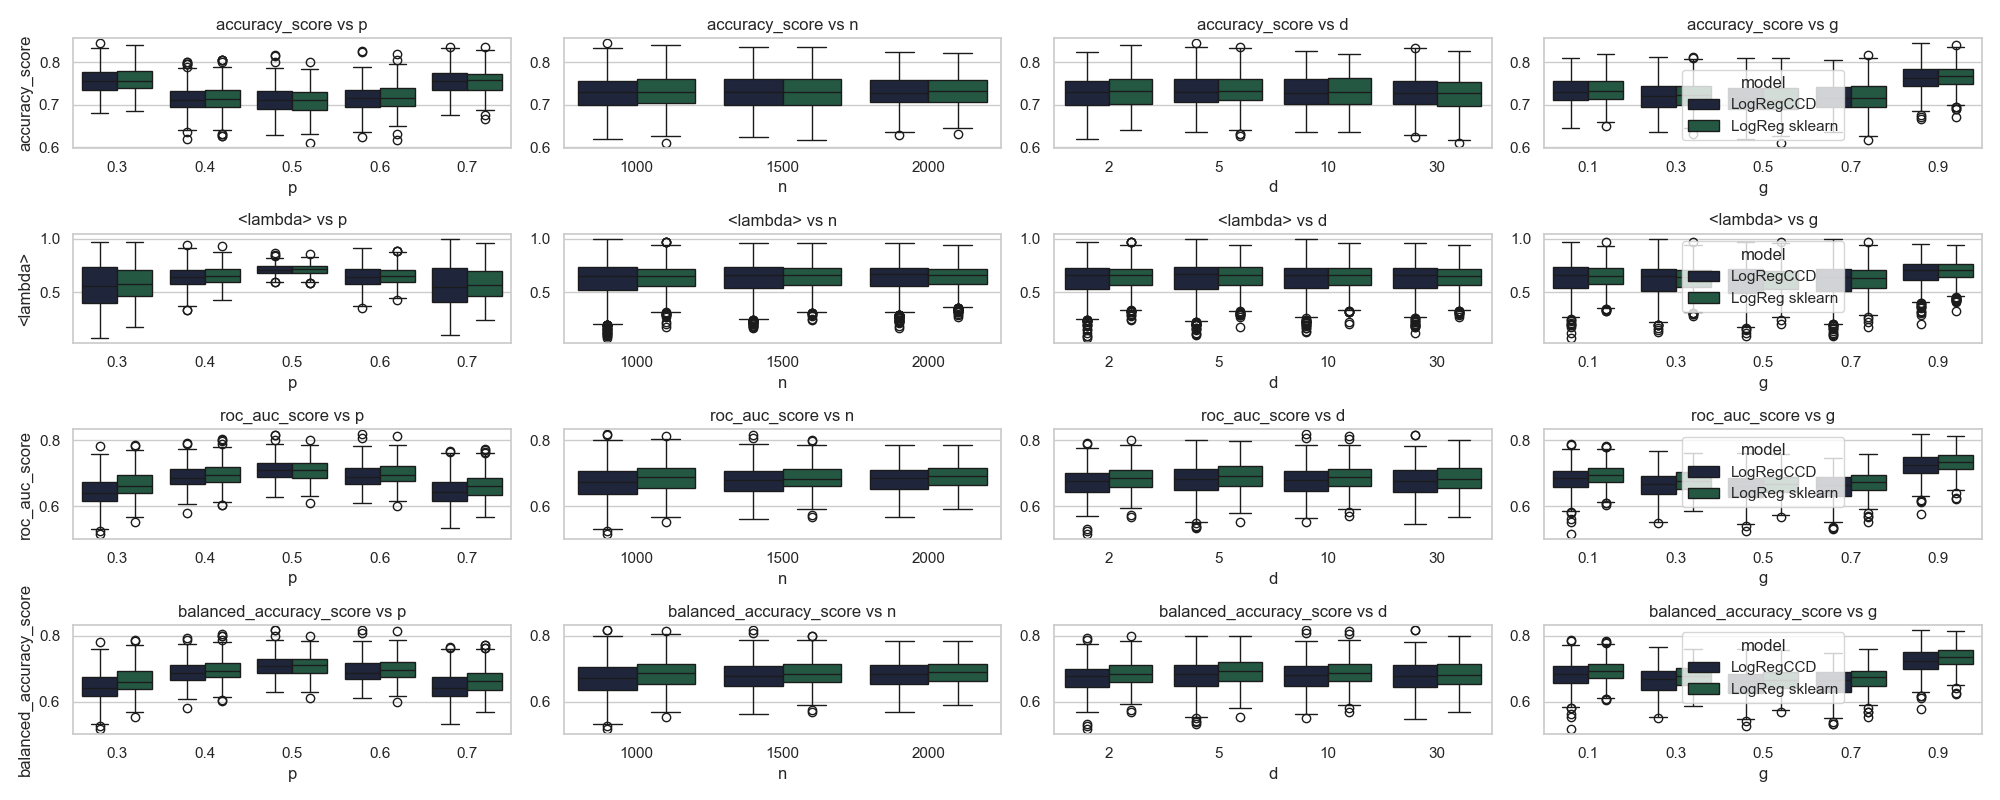
\includegraphics[width=\textwidth]{../results/parameter_facet_grid.png}
    \caption{impact of synthetic dataset parameters on the performance of LogRegCCD algorithm}
    \label{fig:synthetic-dataset-parameters}
  \end{figure}

\section{Benchmark of LogRegCCD with LogisticRegression algorithm}

\subsection{Performance of algorithms regarding different metrics}

\begin{figure}[h]
    \centering
  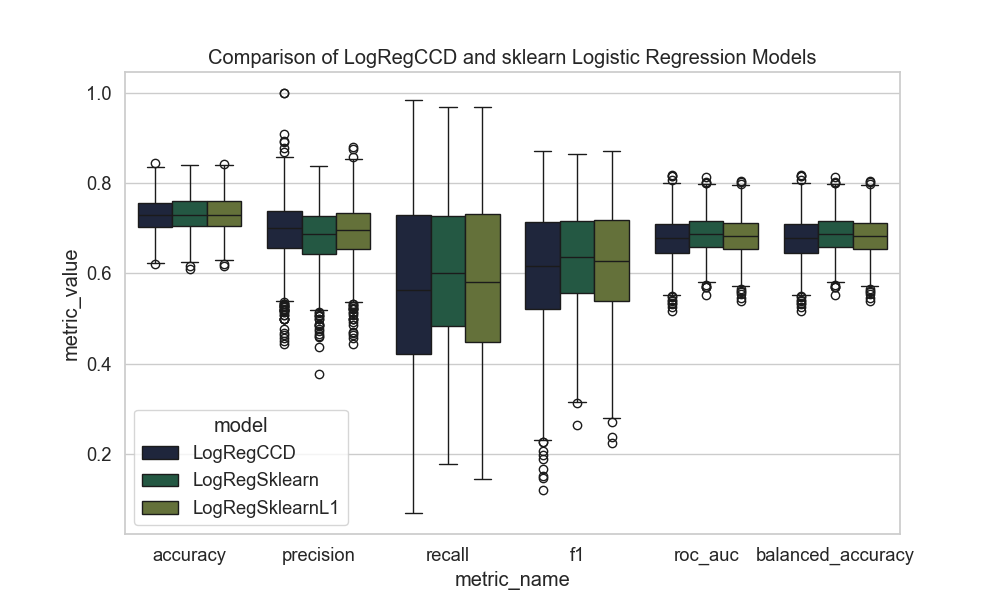
\includegraphics[width=\textwidth]{../results/comparison-synthetic-dataset.png}
    \caption{Comparison of LogRegCCD and LogisticRegression on synthetic dataset}
    \label{fig:comparison-synthetic-dataset}
  \end{figure}

\subsection{Values of coefficients obtained in these two methods}

\section{Discussion about correctness of the LogRegCCD algorithm}

\subsection{Performance of the algorithm at lambda=0}


\begin{figure}[h]
    \centering
    \begin{minipage}{0.48\textwidth}
        \centering
        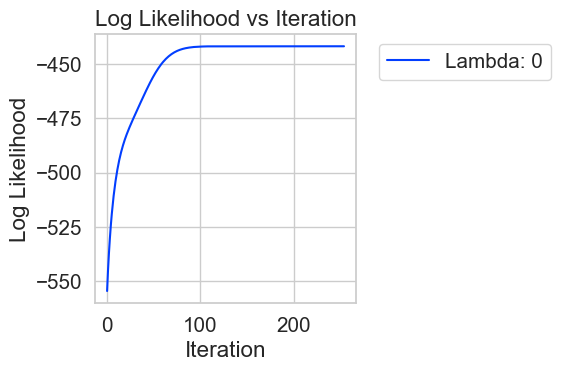
\includegraphics[width=\textwidth]{../results/log_likelihood_synthetic_dataset_lambda_0.png}
        \caption{Log likelihood function values depending on iteration for synthetic dataset with $\lambda=0$}
        \label{fig:log-likelihood-synthetic-dataset-lambda-0}
    \end{minipage}
    \hfill
    \begin{minipage}{0.48\textwidth}
        \centering
        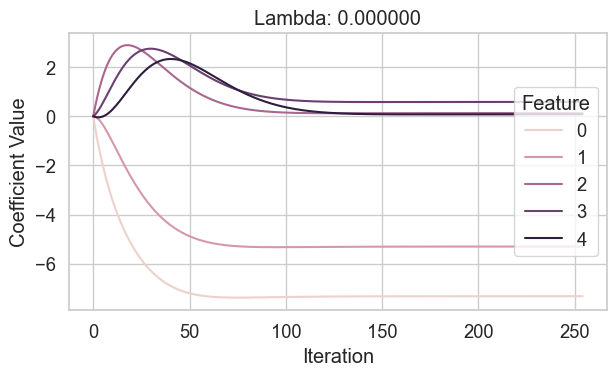
\includegraphics[width=\textwidth]{../results/coefficients_synthetic_dataset_lambda_0.png}
        \caption{Coefficient values depending on iteration for synthetic dataset with $\lambda=0$}
        \label{fig:coefficients-synthetic-dataset-lambda-0}
    \end{minipage}
\end{figure}

\subsection{Likelihood function values and coefficient values depending on iteration}


\begin{figure}
    \centering
  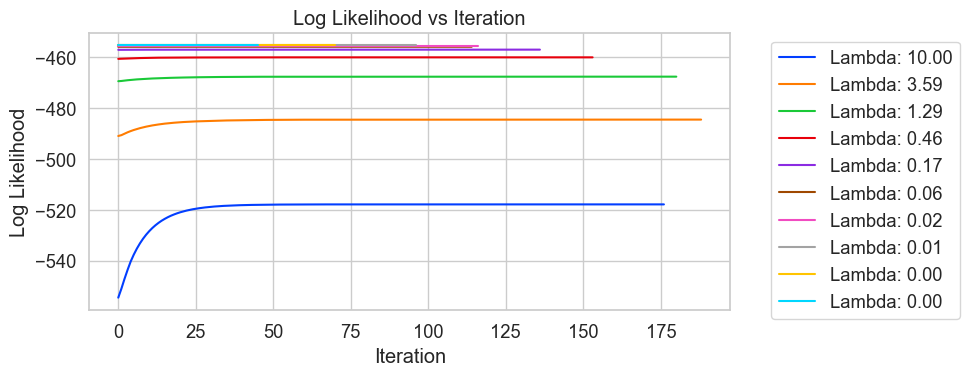
\includegraphics[width=\textwidth]{../results/log_likelihood_synthetic_dataset.png}
    \caption{Log likelihood function values depending on iteration for synthetic dataset}
    \label{fig:log-likelihood-synthetic-dataset}
\end{figure}

\subsection{Comparison with ready implementation of logistic regression with L1 penalty}


\begin{figure}[h]
    \centering
  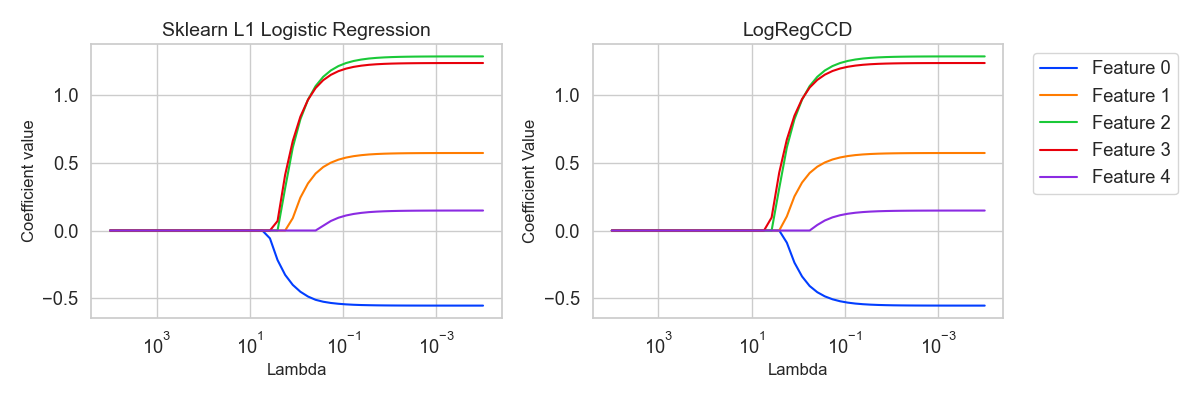
\includegraphics[width=\textwidth]{../results/logistic_regression_l1_logregccd_coefficients_redundant_features.png}
    \caption{Comparison of LogRegCCD and LogisticRegression on synthetic dataset with redundant features}
    \label{fig:comparison-synthetic-dataset-redundant-features}
  \end{figure}


\clearpage 
\listoffigures
\listoftables
\printbibliography

\end{document}
